

\begin{frame}[fragile]{Conjugate Gradients}
 \begin{block}{}
 \begin{center}
  \vspace*{-0.5cm}
  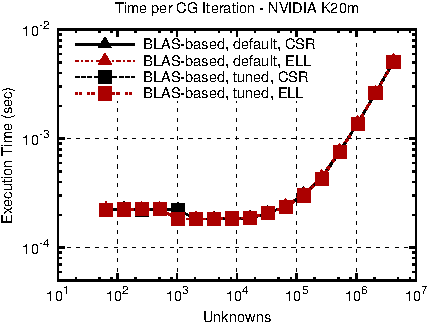
\includegraphics[width=0.85\textwidth]{figures/cg-k20m-2}
 \end{center}

 \begin{itemize}
  \item   \vspace*{-0.3cm} {\small (2D Finite Difference Discretization)}
 \end{itemize}
 \end{block}   
\end{frame}

\begin{frame}[fragile]{Conjugate Gradients}
 \begin{block}{}
 \begin{center}
  \vspace*{-0.5cm}
  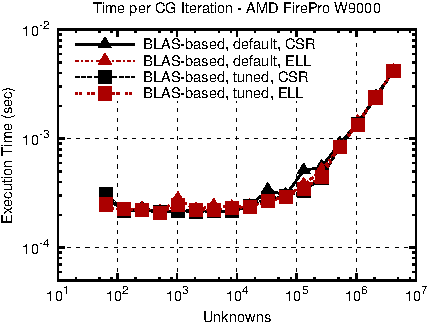
\includegraphics[width=0.85\textwidth]{figures/cg-firepro-w9000-2}
 \end{center}

 \begin{itemize}
  \item   \vspace*{-0.3cm} {\small (2D Finite Difference Discretization)}
 \end{itemize}
 \end{block}   
\end{frame}


% Step 3: Show and discuss pipelined/improved version

\begin{frame}[fragile]{Conjugate Gradient Optimizations}

 \begin{block}{Optimization 3: Rearrange the algorithm}
   \begin{itemize}
   \item  Remove unnecessary reads 
   \item  Remove unnecessary synchronizations
   \item Use custom kernels instead of standard BLAS
  \end{itemize}
 \end{block}
   
\end{frame}


\begin{frame}[fragile]{Conjugate Gradients}

 \begin{block}{}
  
   \begin{minipage}{0.45\textwidth}
      {\large \textbf{Standard CG}} \\
      
      Choose $x_0$ \\
      $p_0 = r_0 = b - Ax_0$ \\
      For $i=0$ until convergence
     \begin{enumerate}
      \item Compute and store $Ap_i$
      \item Compute $\langle p_i, Ap_i \rangle$
      \item $\alpha_i = \langle r_i, r_i \rangle / \langle p_i, Ap_i \rangle$
      \item $x_{i+1} = x_{i} + \alpha_i p_i$          
      \item $r_{i+1} = r_i - \alpha_i Ap_i$       
      \item Compute $\langle r_{i+1}, r_{i+1} \rangle$
      \item $\beta_i = \langle r_{i+1}, r_{i+1} \rangle / \langle r_i, r_i \rangle$
      \item $p_{i+1} = r_{i+1} + \beta_i p_i$
     \end{enumerate}
     EndFor
   \end{minipage}
   \begin{minipage}{0.53\textwidth}
      {\large \textbf{Pipelined CG}} \\
      
      Choose $x_0$ \\
      $p_0 = r_0 = b - Ax_0$ \\
      For $i=1$ until convergence
     \begin{enumerate}
      \item $i=1$: Compute $\alpha_0$, $\beta_0$, $Ap_0$
      \item {\color{blue}$x_i = x_{i-1} + \alpha_{i-1} p_{i-1}$}
      \item {\color{blue}$r_i = r_{i-1} - \alpha_{i-1} Ap_i$}
      \item {\color{blue}$p_i = r_i + \beta_{i-1} p_{i-1}$}       
      \item {\color{red} Compute and store $Ap_i$}
      \item  {\color{red} Compute $\langle Ap_i, Ap_i \rangle$, $\langle p_i, Ap_i \rangle$}, {\color{blue}$\langle r_i, r_i \rangle$}
      \item $\alpha_i = \langle r_i, r_i \rangle / \langle p_i, Ap_i \rangle$
      \item $\beta_i = ( \alpha_i^2 \langle Ap_i, Ap_i \rangle - \langle r_i, r_i \rangle) / \langle r_i, r_i \rangle$
     \end{enumerate}
     EndFor
   \end{minipage}
   
   \end{block}
   
\end{frame}



\begin{frame}[fragile]{Conjugate Gradients}
 \begin{block}{}
 \begin{center}
  \vspace*{-0.5cm}
  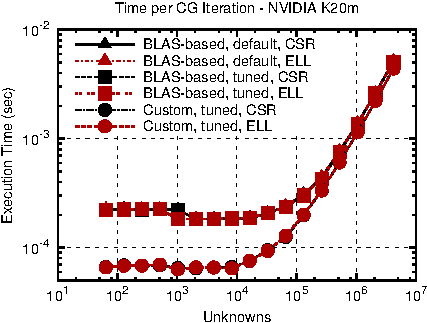
\includegraphics[width=0.85\textwidth]{figures/cg-k20m-3}
 \end{center}

 \begin{itemize}
  \item   \vspace*{-0.3cm} {\small (2D Finite Difference Discretization)}
 \end{itemize}
 \end{block}   
\end{frame}


\begin{frame}[fragile]{Conjugate Gradients}
 \begin{block}{}
 \begin{center}
  \vspace*{-0.5cm}
  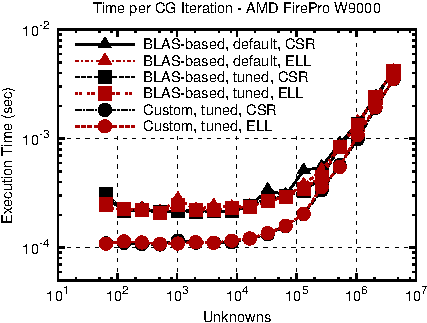
\includegraphics[width=0.85\textwidth]{figures/cg-firepro-w9000-3}
 \end{center}

 \begin{itemize}
  \item   \vspace*{-0.3cm} {\small (2D Finite Difference Discretization)}
 \end{itemize}
 \end{block}   
\end{frame}

\begin{frame}[fragile]{Conjugate Gradients}
 \begin{block}{Benefits of Pipelining also for Large Matrices}
 \begin{center}
  \vspace*{-0.2cm}
  \hspace*{-1.5cm}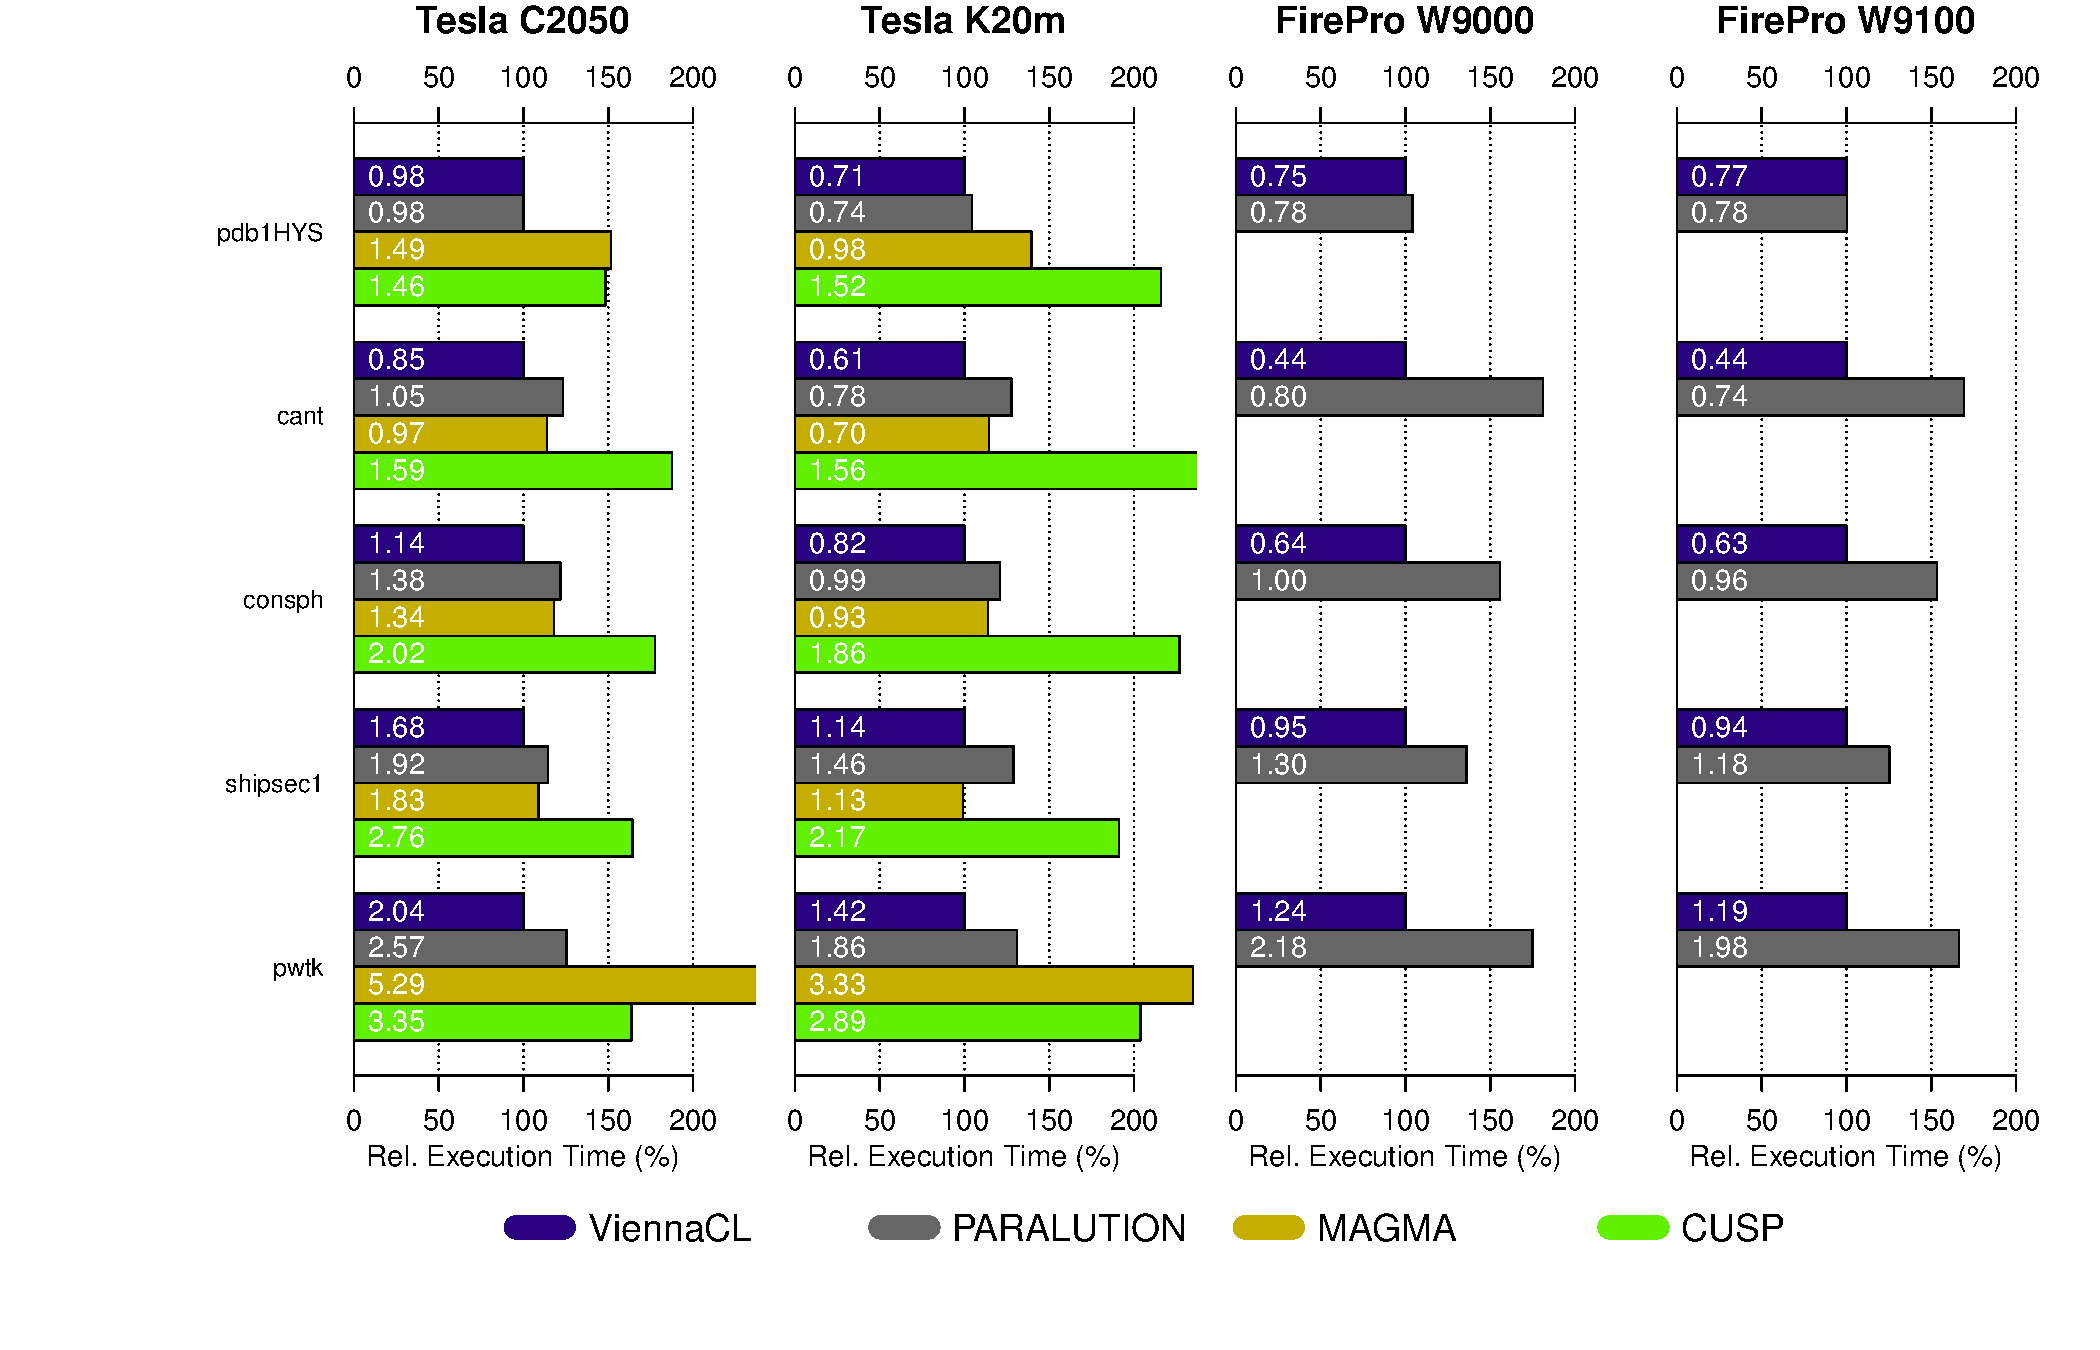
\includegraphics[width=1.05\textwidth]{figures/cg}
 \end{center}
  \vspace*{0.2cm}

 \end{block}   
\end{frame}



